
% ===============================================
% MATH 34: Multivariable calculus           Spring 2019
% hw_template.tex
% ===============================================

% -------------------------------------------------------------------------
% You can ignore this preamble. Go on
% down to the section that says "START HERE" 
% -------------------------------------------------------------------------

\documentclass{article}

\usepackage[margin=1.5in]{geometry} % Please keep the margins at 1.5 so that there is space for grader comments.
\usepackage{amsmath,amsthm,amssymb,hyperref}
\usepackage{graphicx}
\usepackage{float}
\usepackage{listings}
\usepackage{xparse}
\usepackage{xcolor}
\usepackage{verbatim}

\newcommand{\R}{\mathbf{R}}  
\newcommand{\Z}{\mathbf{Z}}
\newcommand{\N}{\mathbf{N}}
\newcommand{\Q}{\mathbf{Q}}
\newcommand{\C}{\mathbf{C}}
\newcommand{\Log}{\text{Log}}
\newcommand{\Arg}{\text{Arg}}
\newcommand{\Real}{\text{Re}}
\newcommand{\Imag}{\text{Im}}

\newenvironment{theorem}[2][Theorem]{\begin{trivlist}
\item[\hskip \labelsep {\bfseries #1}\hskip \labelsep {\bfseries #2.}]}{\end{trivlist}}
\newenvironment{lemma}[2][Lemma]{\begin{trivlist}
\item[\hskip \labelsep {\bfseries #1}\hskip \labelsep {\bfseries #2.}]}{\end{trivlist}}
\newenvironment{claim}[2][Claim]{\begin{trivlist}
\item[\hskip \labelsep {\bfseries #1}\hskip \labelsep {\bfseries #2.}]}{\end{trivlist}}
\newenvironment{problem}[2][Problem]{\begin{trivlist}
\item[\hskip \labelsep {\bfseries #1}\hskip \labelsep {\bfseries #2.}]}{\end{trivlist}}
\newenvironment{proposition}[2][Proposition]{\begin{trivlist}
\item[\hskip \labelsep {\bfseries #1}\hskip \labelsep {\bfseries #2.}]}{\end{trivlist}}
\newenvironment{corollary}[2][Corollary]{\begin{trivlist}
\item[\hskip \labelsep {\bfseries #1}\hskip \labelsep {\bfseries #2.}]}{\end{trivlist}}

\newenvironment{solution}{\begin{proof}[Solution]}{\end{proof}}

\makeatletter
\newcommand{\skipitems}[1]{%
	\addtocounter{\@enumctr}{#1}%
}
\makeatother

\NewDocumentCommand{\codeword}{v}{%
\texttt{\textcolor{blue}{#1}}%
}


\begin{document}

\large % please keep the text at this size for ease of reading.

% ------------------------------------------ %
%                 START HERE             %
% ------------------------------------------ %

{\Large Page 1 % Replace with appropriate page number 
\hfill  MTH483, Complex Variables, HW4}

\begin{center}
{\Large Wyatt Whiting}
\end{center}
\vspace{0.05in}

% -----------------------------------------------------
% The "enumerate" environment allows for automatic problem numbering.
% To make the number for the next problem, type " \item ". 
% To make sub-problems such as (a), (b), etc., use an "enumerate" within an "enumerate."
% -----------------------------------------------------
\begin{enumerate}

%%Problem 1
	\item $G = \{z \in \C: |z|<2 \text{ and } \Real(z^2)\leq 1 \}$
		\begin{enumerate}
			\item \codeword{RegionPlot[Abs[x + I y] < 2 && Re[(x + I y)^2] <= 1, {x, -3, 3}, {y, -3, 3}]}
			\begin{figure}[H]
			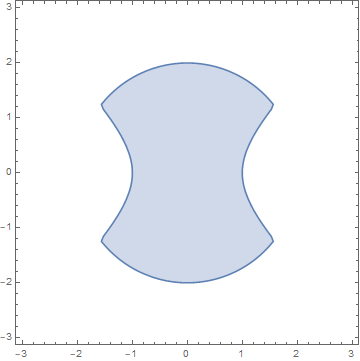
\includegraphics[scale=0.5]{image1.png}
			\end{figure}
			The region does not contain the upper or lower convex curves or their endpoints, but does contain the concave curves on the sides of the region.
			
			\item Interior points: $\{z \in \C: |z|<2 \text{ and } \Real(z^2) < 1 \}$
			\item Boundary points: I wasn't able to come up with a closed set to describe the boundary, but it is the line surrounding the region including the corners. The following figure highlights the set of boundary points in red.
			
			\codeword{RegionPlot[Abs[x + I y] < 2 && Re[(x + I y)^2] <= 1, {x, -3, 3}, {y, -3, 3}, BoundaryStyle -> Directive[Red, Bold]]}
			\begin{figure}[H]
			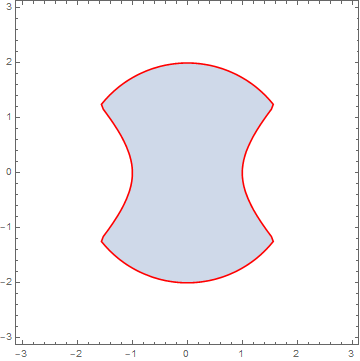
\includegraphics[scale=0.4]{image2.png}
			\end{figure}
			
			\item G is neither open nor closed. We may construct a sequence of complex number which converge to $z=2i$, but $z=2i$ is not in the region, so it cannot be closed. It is not open because $z=1+0i$ is in G, but no circle around this point will be entirely within G. Thus, G is neither open nor closed.
		\end{enumerate}
		
%%Problem 2
	\item To each of the following functions, determine the region of continuity. 
		\begin{enumerate}
			\item $f(z)=\overline{z}$
			
			$f(z)=\overline{z}=\overline{a+bi}=a-bi$. So then given an arbitrary $z_0 \in \C$,
		 $$\lim_{z\to z_0}f(z)=\lim_{a\to a_0}a - \lim_{b\to b_0}bi=a_0-b_0 i.$$
		 Each component is continuous on $\C$, so $f(z)=\overline{z}$ is continuous on $\C$ as well.
		 
		 \item $f(z)=|z|$
		 
		 We have 
		 $$\lim_{z\to z_0}f(z)=\lim_{r\to r_0}\lim_{\theta \to \theta_0}|re^{i\theta}|=\lim_{r\to r_0}r = r_0$$
		 
		 It intuitively makes sense that this function is continuous on all of $\C$ since the modulus function has no jump discontinuities; the modulus of a complex number varies smoothly between any two points.
		 
		 \item $f(z)=\sinh(z)$
		 
		 We have $f(z)=\sinh(a+bi)=\sinh(a)\cos(b)+i\cosh(a)\sin(b) $. So then
		 
		 $$f(z)=\sinh(a+bi)=\frac{e^a-e^{-a}}{2}\cos(b)+i\left(\frac{e^a+e^{-a}}{2}\sin(b)\right) $$
		 We know that $\sin$ and $\cos$ are continuous for all real values, and we also know that both $\frac{e^a-e^{-a}}{2}$ and $\frac{e^a-e^{-a}}{2}$ are continuous for all real values as well. Thus the products $\frac{e^a-e^{-a}}{2}\cos(b)$ and $\frac{e^a+e^{-a}}{2}\sin(b) $ are both continuous for any $a,b\in \R$. Therefore, we may conclude that $f(z)=\sinh(z)$ is continuous on $\C$.
		 \item $f(z)=(z+1)^{1/2}$
		 We know that $f(z)=(z+1)^{1/2}=e^{\ln|z+1|+i\Arg(z+1)}$, and the region of continuity of the $\Arg$ function is $\C\setminus \R_{\leqslant 0}$. By adding 1 to the argument, the region of continuity is effectively shifted in the negative real direction by 1 unit. Thus, the region of continuity of $f(z)=(z+1)^{1/2}$ is $\C\setminus\R_{\leqslant -1}$.
		 
		 \item $f(z)=\Log(z-i)+\Log(z+i)$
		 
		 Each $\Log$ term has its own region of continuity. We are using $\Log$ and not $\log$, so we use the principle branch of the function. Subtracting $i$ from the $z$ has the effect of moving the region of continuity of $\Log(z-i)$ by $+i$ units relative to $\Log(z)$, so the region of continuity of $Log(z-i)$ is $\{z = a+bi \in\C : a\in\R_{\leqslant 0}, b=1 \}$. By a parallel argument, the region of continuity of $\Log(z+i)$ is $\{z=a+bi\in\C : a=\R_{\leqslant 0}, b=-1 \}$. Thus, the region of continuity of $f(z) = \C\setminus\{z=a+bi\in\C : a \leqslant 0 \text{ and } (b = 1 \text{ or } b=-1)\}$
		\end{enumerate}

%%Problem 3		
	\item Find a parametrization for each of the following curves:
		\begin{enumerate}
			\item The circle centered at $1+i$ with radius 3
			
			\[\{ (3\cos(t)+1)+i(3\sin(t)+1)\in\C : 0 \leqslant t \leq 2\pi \}\]
			
			\item The line segment from $-1-i$ to $2i$.
			\[\{ (-1+t)+i(-1+3t)\in\C : 0\leqslant t \leqslant 1 \}\]
			
			\item The infinite line passing through $1-2i$ and $2+i$
			
			\[\{ (1+t)+i(-2+3t)\in\C : -\infty < t < \infty \}\]
			
			\item The upper half of the circle centered at $-1+i$ with radius $2$ oriented clockwise.
			\[\{ (-2\cos(t)-1)+i(2\sin(t)+1)\in\C : 0 \leqslant t \leqslant \pi \}\]
		\end{enumerate}
		
	\skipitems{1}
		
	\item Consider the multivalued function $g(z)=\log(z^3+1)$	 
		\begin{enumerate}
			\item $\log(z^3+1)=\ln|z^3+1|+i\arg(z^3+1)$, so $\Real(g(z))=\ln|z^3+1|$ and $\Imag(g(z))=\arg(z^3+1)$.
			
			\item \codeword{g[z_] := Log[z^3 + 1]}
			
			\codeword{ParametricPlot3D[{x, y, Re[g[x + I y]]}, {x, -5, 5}, {y, -5, 5}]}
			\begin{figure}[H]
			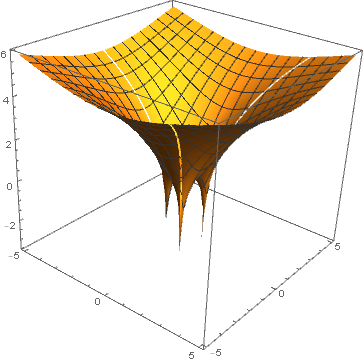
\includegraphics[scale=0.7]{image3.png}
			\end{figure}
			\item $F(z)=\Arg(z^3 + 1)$
			
			
			\item \codeword{ParametricPlot3D[{x, y, Arg[(x + I y)^3 + 1]}, {x, -5, 5}, {y, -5, 5}]}
			\begin{figure}[H]
			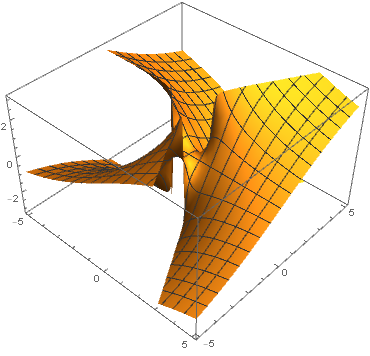
\includegraphics[scale=0.7]{image4.png}
			\end{figure}
			
			\[ F(1+i)=\Arg((1+i)^3+1)=Arg(-1+2i)=\arctan(-2)+\pi\]
			
			\item The branch cuts in the complex plane are three rays pointing radially away from the origin with endpoints evenly distributed around the origin such that the rays are symmetric over the real axis. The branch points are the endpoints of the rays.
			
			\item Let B denote the set of branch points. Then,
			
			\[ B = \{ e^{-i\frac{\pi}{3}}, e^{i\frac{\pi}{3}},e^{i\pi} \} \]
		
		\item The branch cuts are represented by the paths:
		
		\[\gamma_1:= te^{-i\frac{\pi}{3}}; \]
		\[\gamma_2:= te^{i\frac{\pi}{3}}; \]
		\[\gamma_3:= te^{i\pi}; \]
		
		where $t \geq 1$ in each path.
		
		\item \codeword{p[k_] := Plot3D[Arg[(x + I y)^3 + 1] + Pi*2*k, {x, -5, 5}, {y, -5, 5}]}
		\codeword{Show[p[-1], p[0], p[1], PlotRange -> All]}
		\begin{figure}[H]
		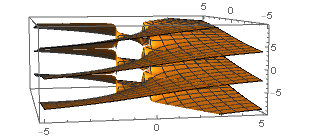
\includegraphics[scale=0.8]{image5.png}
		\end{figure}
		The figure was rotated from its default view in order to show the multivalued property of the function $f(z)$.
		\end{enumerate}
\end{enumerate}

% ---------------------------------------------------
% Anything after the \end{document} will be ignored by the typesetting.
% ----------------------------------------------------

\end{document}

